\chapter{Driver de la commande des moteurs}

\section{Rappel}

Le driver moteur a pour mission de permettre de contrôler les moteurs de rotation, inclinaison et zoom du télescope. Mais également assurer la sécurité du système de pilotage à bas niveau. Le système de sécurité consiste à interrompre le mouvement d’inclinaison ou de zoom si ils atteignent leur fin de course.

\section{Fonctionnalités}

\begin{figure}[H]
    \centering
    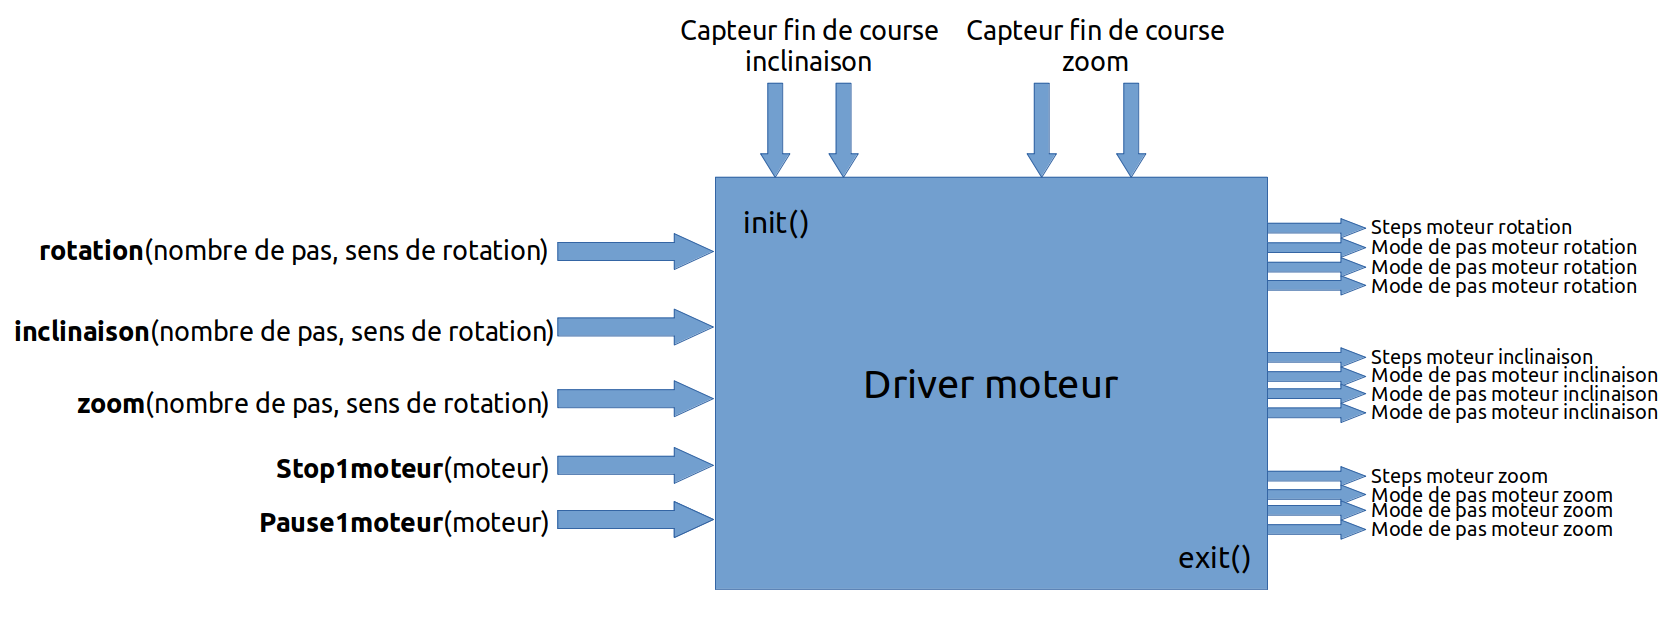
\includegraphics[width=1\linewidth]{\figures/sch_driver_motor.png}
    \decoRule
    \caption[
    Schéma des entrées / sorties du driver moteur]{
    Schéma des entrées / sorties du driver moteur}
    \label{fig:Schéma des entrées / sorties du driver moteur}
    \end{figure}

\vspace{1cm}

Le driver va permettre l’utilisation des fonctions qui se trouvent à gauche du bloc "driver moteur". Chacune des fonctions agit sur les sorties. Les capteurs de fin de course servent de sécurité, cette partie est indépendante du reste et arrête le moteur qui à atteint sa position de butée.
Les sorties "mode de pas moteur..." permettent de choisir dans quel mode de rotation doit tourner le moteur (pas complet, demi-pas, quart de pas, huitième de pas, seizième de pas). Réduire la division de pas permet d’affiner la rotation afin d’atteindre l’angle le plus exact possible à ce qui à été commandé.

\section{Câblage}

\begin{figure}[H]
    \centering
    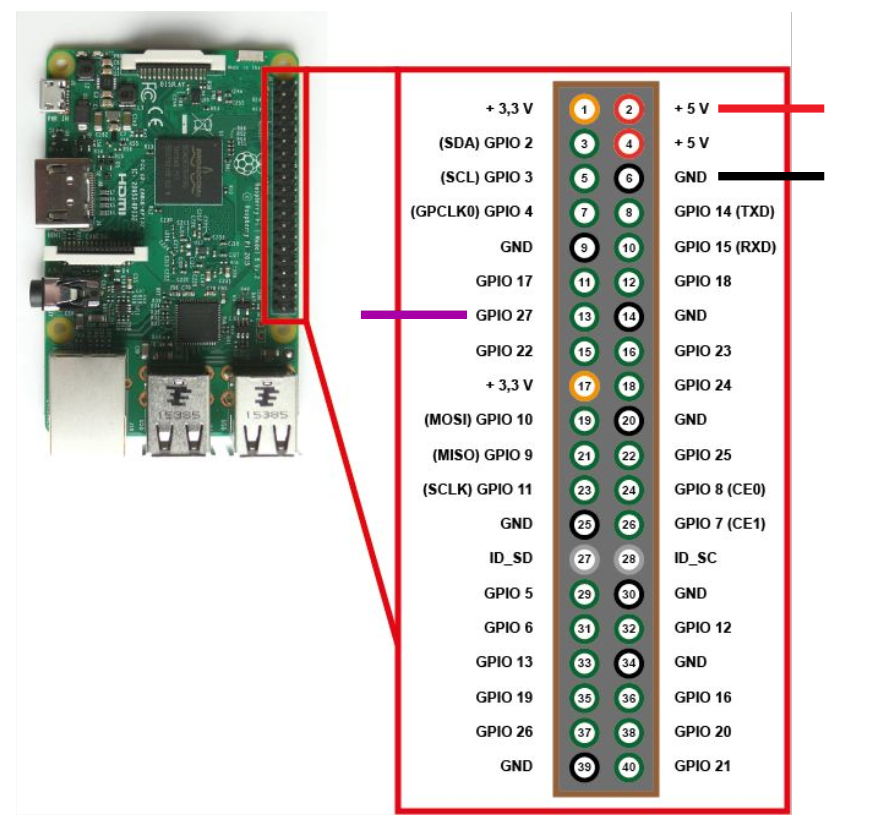
\includegraphics[width=0.5\linewidth]{\figures/sch_pinout.png}
    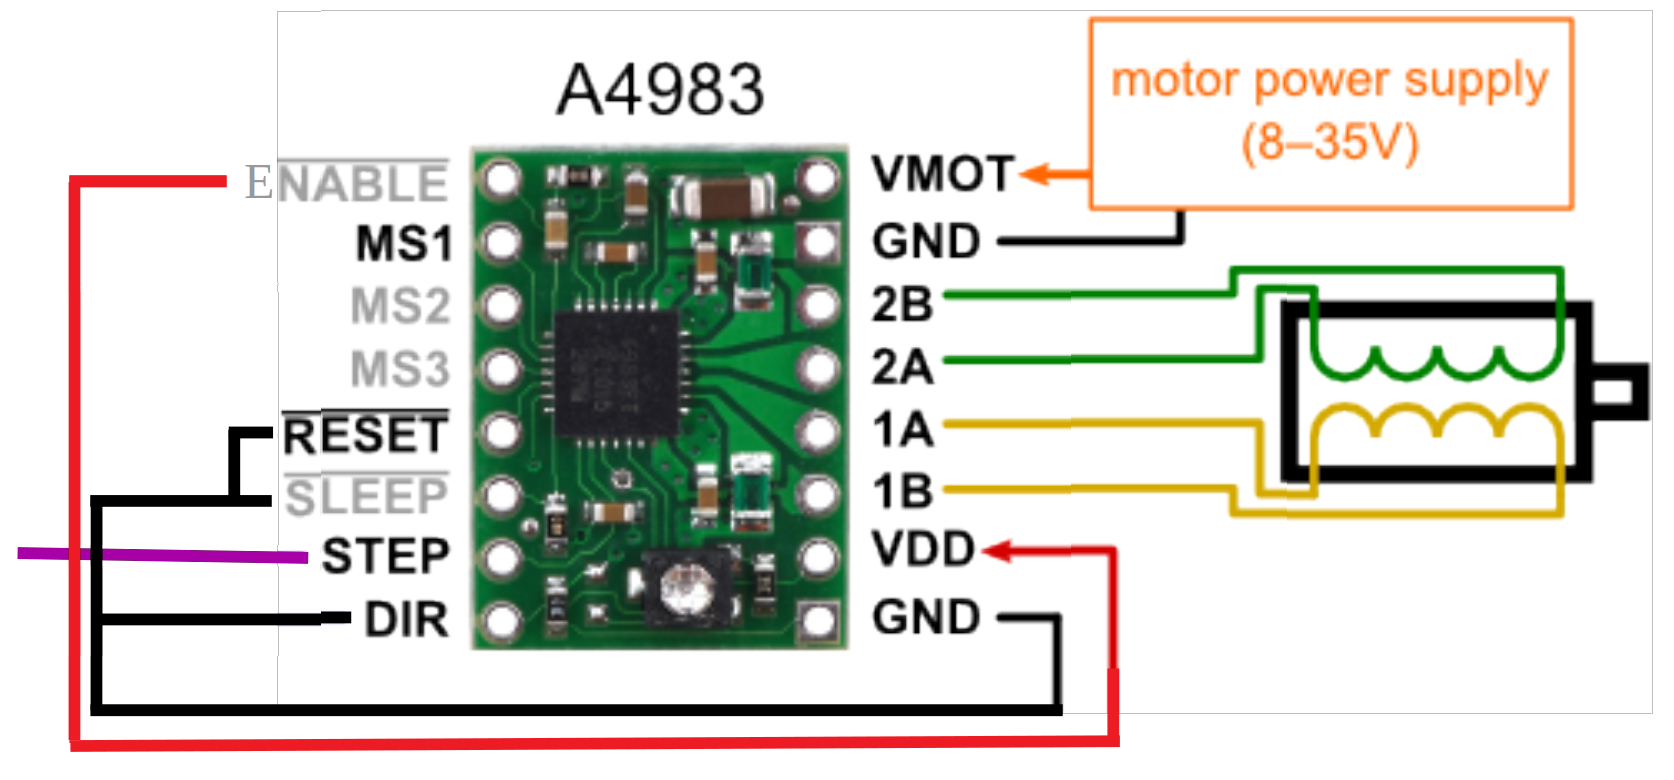
\includegraphics[width=0.5\linewidth]{\figures/sch_a4983.png}
    \decoRule
    \caption[
    Schéma de câblage d'un contrôleur moteur sur la Raspberry Pi]{
    Schéma de câblage d'un contrôleur moteur sur la Raspberry Pi}
    \label{fig:Schéma de câblage d'un contrôleur moteur sur la Raspberry Pi}
    \end{figure}

\section{Avancement du programme}

La première version du driver qui est validé depuis fin janvier permet~:
\begin{itemize}[label=$\bullet$]
	\item Initialiser le driver
	\item Lancer la rotation (à 5ms max par période de step)
	\item Lancer l’inclinaison (à 5ms max par période de step)
	\item Stopper les moteurs grâce aux capteurs de fin de course
	\end{itemize}

\vspace{1cm}

À suivre~:
\begin{itemize}[label=$\bullet$]
	\item La partie qui consiste à changer de mode de pas est codé mais pas testé.
	\item Étendre le système pour gérer le zoom.
	\end{itemize}

\section{Procédure de test}

Pour valider mon driver, je l’ai testé avec une Raspberry Pi, un contrôleur moteur et un moteur.

\begin{figure}[H]
    \centering
    \includegraphics[width=0.9\linewidth]{\figures/photo_test_motor.jpg}
    \decoRule
    \caption[
    Photo du banc de test]{
	Photo du banc de test}
    \label{fig:Photo du banc de test}
    \end{figure}

\vspace{1cm}

J’ai pu valider les fonctionnalités développées, cependant la vitesse max atteinte par le moteur contrôlé par le driver est inférieure à celle que l'on peut atteindre en contrôlant le moteur avec un générateur basse fréquence.
Voici le résultat de la commande envoyée par la Raspberry Pi par la pin Step au contrôleur moteur pour faire avancer à chaque front montant le moteur de 1 pas.

\begin{figure}[H]
    \centering
    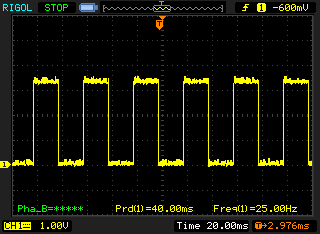
\includegraphics[width=0.5\linewidth]{\figures/osc_motor.png}
    \decoRule
    \caption[
    Mesure à l'oscilloscope de la commande moteur générée]{
	Mesure à l'oscilloscope de la commande moteur générée}
    \label{fig:Mesure à l'oscilloscope de la commande moteur générée}
    \end{figure}

\vspace{1cm}

Après avoir étudié les résultats avec d'autres professeurs, j'ai conclu que la période minimale que je puisse atteindre soit de $20ms$ est normal. Cette limitation est due au fait que mon driver n'a pas la priorité des ressources dans le Linux. Et que le Linux a un cycle lecture/écriture des entrées/sorties limité. Pour améliorer cela il faudrait passer sur un Linux temps réel.

\section{Interactions avec le driver}

Le driver devra pourvoir être utilisé à partir d'une application situé dans le user-space du linux embarqué. Pour cela j'ai étudié et testé plusieurs solutions.

Le première qui m'est venu à l'idée était d'utiliser l'IPC (inter process communication). 

Une seconde plus archaïque m'est venu à l'idée, celle de partager un ficher entre le programme dans le user-space et du driver. Pour que le programme dans le user-space puisse transférer ses ordres. Cependant je trouve cette solution pas très sécuritaire.

La troisième solution qui m'a été proposé par Vincent Poulailleau est d'utiliser la fonction ioctrl. C'est cette solution que j'ai retenu car elle est une technique très rodé dans le domaine car elle était déjà utilisé à la version 7 d'UNIX. 

\vspace{1cm}

Je suis maintenant en phase de développement de cette fonction pour l'ajouter au driver existant.


